\documentclass{article}
\usepackage{lscape}
\usepackage{lipsum}
\usepackage[margin=1in,includefoot]{geometry}
\usepackage{graphicx}
\usepackage{float}
\usepackage{amsmath}
\usepackage{amssymb}

% Header and Footer Stuff
\usepackage{fancyhdr}
\pagestyle{fancy}
\fancyhead{}
\fancyfoot{}
\fancyfoot[R]{\thepage}
\renewcommand{\headrulewidth}{0pt}
\renewcommand{\footrulewidth}{0pt}

\begin{document}

\begin{titlepage}
	\begin{center}
	\begin{align*}
	
\includegraphics[height=1.75in]{logo.png}
	\end{align*}


	
	\line(1,0){300}\\
	[0.25in]
	\huge{\bfseries Business Plan}\\
	[2mm]
	\line(1,0){200}\\
	[1.5cm]
	
	\textsc{\Large 3E4 Management For Engineering}\\
	[7cm]	
	\end{center}
	
	
	
	\begin{flushright}
	\
	08 April 2016\\}
	\end{flushright}

\end{titlepage}
%Table of Contents Stuff%
\tableofcontents
%\listoffigures
%\addcontentsline{toc}{section}{List of Figures}
\listoftables
\addcontentsline{toc}{section}{List of Tables}


\thispagestyle{empty}
\cleardoublepage
\pagenumbering{arabic}
\setcounter{page}{1}


\section{Executive Summary}\label{sec:intro}

MEDVAC is a specialised lathroscopy product aimed at making surgeries safer, faster and more transparent. The product aims to increase efficiency in surgery, as well as providing a means of helping to increase the quality of education provided to the field.




\begin{align*}
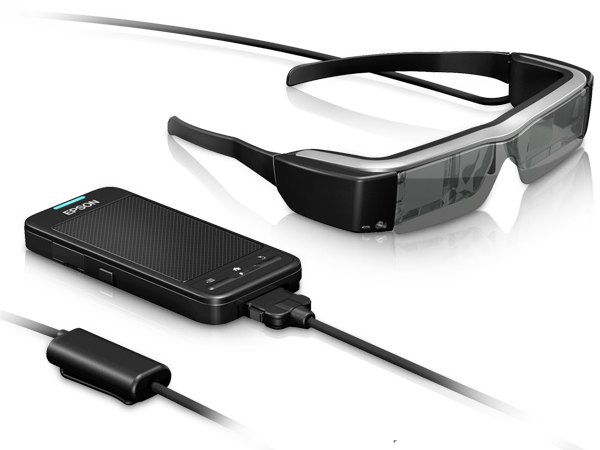
\includegraphics[height=1.75in]{concept2.png}
\end{align*}\\









\begin{align*}
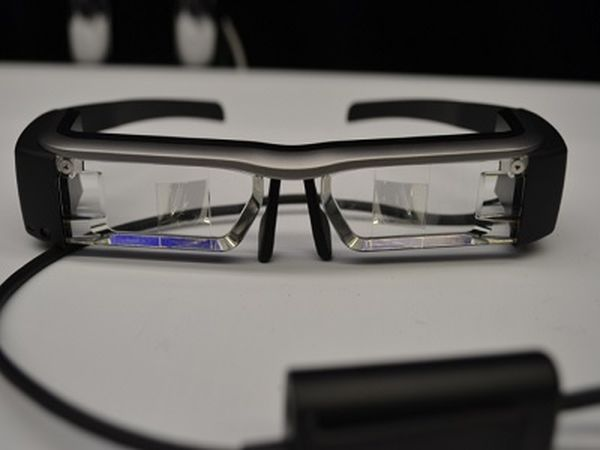
\includegraphics[height=1.75in]{concept3.jpg}
\end{align*}\\


\begin{align*}
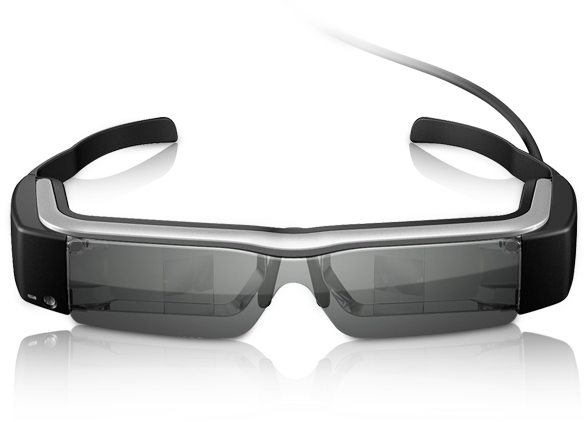
\includegraphics[height=1.75in]{concept4.png}
\end{align*}\\


\section{In- Depth Summary}
The optics and image techniques in the surgery field have a very important role. Before a surgery, structural or functional images are required in order to focalise where the pathogenic mechanism is occurring. In the case of laparoscopy and endoscopy, in which they are the eyes of the surgeon. However, the surgeon must divert attention to look at the screen to see this information or to be able to follow the surgery. For this reason, a head display will be useful and also can act as diagnosis tool in real time. The head-up display will be based on a number of principal.

The heads up display seeks to constantly update the surgeon on the patient's vitals as to minimize fatigue and make it more comfortable for the surgeon to operate.

Secondly, using a sensitive camera sensor, the patient's vital blood vessels can also be detected, mapped, and displayed in the augmented-reality display system. This is to alarm  the surgeon of possible dangers in a given situation of operation, such as cutting below that tissue, or to show the surgeon where and how deep that vessel is.

Thirdly the system would function as a recording system for hospitals, hopefully reducing the insurance cost of hospitals and the amount of legal difficulties associated with an unsatisfactory end to a surgery, or forgotten equipment within a patient, which has previously happened in various cases.

Finally, the display would serve as a guide and teaching apparatus for new surgeons to see how a surgery is operator or for experienced surgeons to examine past surgeries and improve on the standard of care given, thus allowing future surgeons to learn on a much more intimate level of knowledge, as the perspective of the viewing is different from simply that of an onlooker.






\section{Target Customers}
Our customer profile is a surgeon, either that of a trainee being educated in university, all the way up to an experienced surgeon who would use this product to increase the efficiency of work, and reap the rewards of its advantages of use. The profile is a well educated individual who wants to become more experienced in the field of surgery, and spends the majority of their day seeking to improve the lives of patients through medical practice. Hospitals and universities are examples of workplaces or places of use where the product would be aimed for use.




\pagebreak

\section{Unique Selling Proposition}
Our unique selling proposition is simple - make the world a better place. Surgery and healthcare are key aspects to a satisfied society. We strive to build on this and help patients get the best care that they deserve and are entitled to receive. 





\section{Pricing & Positioning Strategy}
Our pricing structure is based primarily on a licence methodology, which allows us to keep regular contact with clients of our product. As well as this, it allows for a regular and steady income whereby smaller, regular sales are received instead of relying on a larger once off, or annual pricing structure where the client and our business are only in contact seldom. This pricing structure gives a greater sense of stability in the company and ensures that clients are more easily accessible due to the nature of paying less up front, with the possibility and ease of mind for the client to simply cancel a subscription if necessary. With this in mind, it’s possible to quickly know which organisations are still interested in long term use of our product, and therefore cuts down on the amount of uncertainty of whether or not new clients should be sought after at a given moment.




\section{Distribution Plan}
Our distribution plan is primarily based on a face to face set of meetings, with clients being vetted first. Preapproved and well known hospitals and organisations are key to ensuring that our reputation grows as a result with professionalism. Distributions will namely be on a licence or contract based strategy, ergo allowing use of our product on short or long term intervals, which are governed by many consecutive time periods the client pays for.






\section{Online Marketing Strategy}

The four key components to your online marketing strategy are as follows:
Keyword Strategy: identify what keywords you would like to optimize your website for.
Search Engine Optimization Strategy: document updates you will make to your website so it shows up more prominently for your top keywords.
Paid Online Advertising Strategy: write down the online advertising programs will you use to reach target customers.
Social Media Strategy: document how you will use social media websites to attract customers.

-Online marketing strategy-
The keywords we would like to optimize our product would be solution, cutting edge, surgery, efficiency, etc
We aim to structure our website so that our name and reputation are first to appear on searches with certifications from recommended clients
We will take out multiple advertisements describing our business and what we can deliver to hospitals and researchers
We will set up online accounts tiered towards research groups to promote our product as a business to business product, as social media is unsuitable for promoting such a specialised and research driven product. Aims would be put in place to tackle expanding contacts and potential clients via universities and hospitals.





\section{Distribution Plan}



\section{Conversion Strategy}
The conversion plan for our venture hinges on the delivery of good customer relations and quality service. By delivering a quality service to our customers we will make ourselves integral to their expansion and growth plans and thus paying for a licensing fee will not seem as complicated or expensive.

\section{Benefits}
Due to the complexity and cost of the device it can only ever be a B to B model as the average person would generally not have a need for a highly specialised lathroscopic device.
B to B model is more reliable as the attrition of customers is not as high. The feedback from customers is also more personal. The customer relationship is also better as the clients interact with us on a monthly basis.
Our product is secure from imitation or patent theft or infringement as the company will know the location of all the devices in use around the world. This careful and extended vice does not end up in the w=knowledge of our customers will ensure that our device does not end up in the wrong hands.

\section{Financial Projections}


\subsection{Overheads}
\begin{table}[H]
\centering
\caption{Overheads}
\label{my-label}
\begin{tabular}{llll}
Write your business name here     &        & MEDVAC &        \\
                                  &        &        &        \\
                                  &        &        &        \\
OPERATING BUDGET                  &        &        &        \\
ANALYSIS OF OVERHEADS             &        &        &        \\
                                  &        &        &        \\
                                  & Year 1 & Year 2 & Year 3 \\
                                  & €      & €      & €      \\
                                  &        &        &        \\
Staff costs                       &        &        &        \\
Gross staff salaries              & 0      & 40000 & 40000 \\
Employer’s PRSI                   & 0      & 5000   & 7000   \\
Bonuses, etc.                     & 0      & 10000  & 10500  \\
Staff training costs              & 0      & 1000   & 1500   \\
Other staff costs                 & 0      & 0      & 0      \\
Total staff costs                 & 0      & 56000 & 59000 \\
                                  &        &        &        \\
Production overheads              &        &        &        \\
Use of auxiliary materials        & 0      & 500    & 1000   \\
Maintenance                       & 0      & 0      & 0      \\
Heat, light \& power              & 0      & 0      & 0      \\
Rent/lease of equipment           & 0      & 0      & 0      \\
Insurance on equipment            & 0      & 0      & 0      \\
Other costs                       & 0      & 0      & 0      \\
Total production costs            & 0      & 500    & 1000   \\
                                  &        &        &        \\
Premises costs                    &        &        &        \\
Rent                              & 0      & 7200   & 7200   \\
Heat, light \& power              & 0      & 0      & 0      \\
Insurance                         & 0      & 0      & 0      \\
Cleaning                          & 0      & 500    & 700    \\
Maintenance                       & 0      & 0      & 0      \\
Other costs                       & 50     & 100    & 300    \\
Deduct:                           & 0      & 0      & 0      \\
Rent received                     & 0      & 0      & 0      \\
Total premises costs              & 50     & 7800   & 8200   \\
                                  &        &        &        \\
Transport costs                   &        &        &        \\
Maintenance and repairs           & 0      & 0      & 0      \\
Lease costs                       & 0      & 0      & 0      \\
Fuel                              & 0      & 0      & 0      \\
Insurance                         & 0      & 0      & 0      \\
Road Tax                          & 0      & 0      & 0      \\
Public transport                  & 0      & 0      & 0      \\
Air fares                         & 0      & 0      & 0      \\
Deduct:                           & 0      & 0      & 0      \\
Private use                       & 0      & 0      & 0      \\
Total transport costs             & 0      & 0      & 0      \\
                                  &        &        &        \\
Selling and promotion costs       &        &        &        \\
Advertising                       & 0      & 1500   & 1500   \\
Packaging                         & 0      & 0      & 0      \\
Promotion                         & 0      & 0      & 500    \\
Trade fairs                       & 0      & 0      & 0      \\
Commissions                       & 0      & 0      & 0      \\
Other costs                       & 0      & 0      & 0      \\
Total selling and promotion costs & 0      & 1500   & 2000   \\
                                  &        &        &        \\
General expenses                  &        &        &        \\
Telephone                         & 0      & 0      & 0      \\
Postage                           & 50     & 50     & 50     \\
Subscriptions                     & 0      & 0      & 0      \\
Insurance                         & 0      & 0      & 0      \\
Stationery                        & 100    & 100    & 100    \\
Office expenses                   & 0      & 500    & 1000   \\
Accountancy fees                  & 300    & 300    & 300    \\
Legal \& other fees               & 800    & 800    & 800    \\
Other costs                       & 0      & 0      & 0      \\
Total general expenses            & 1250   & 1750   & 2250   \\
                                  &        &        &        \\
Finance costs                     &        &        &        \\
Interest on loans/overdraft       & 0      & 0      & 0      \\
Mortgage interest                 & 0      & 0      & 0      \\
Charges/fees                      & 0      & 0      & 0      \\
Other                             & 0      & 0      & 0      \\
Total finance costs               & 0      & 0      & 0      \\
                                  &        &        &        \\
Depreciation                      &        &        &        \\
Property                          & 0      & 0      & 0      \\
Fixtures \& fittings              & 0      & 0      & 0      \\
Transport                         & 0      & 0      & 0      \\
Machines and equipment            & 0      & 0      & 0      \\
Other                             & 0      & 0      & 0      \\
Total depreciation costs          & 0      & 0      & 0      \\
                                  &        &        &        \\
                                  &        &        &        \\
Total Overheads                   & 1300   & 67550 & 72450
\end{tabular}
\end{table}




\subsection{Salesprofit}

\begin{table}[H]
\centering
\caption{Sales Profit}
\label{my-label}
\begin{tabular}{llll}
Write your business name here      & MEDVAC &        &        \\
                                   &        &        &        \\
                                   &        &        &        \\
OPERATING BUDGET                   &        &        &        \\
ESTIMATE OF SALES AND GROSS PROFIT &        &        &        \\
                                   &        &        &        \\
                                   &        &        &        \\
                                   & Year 1 & Year 2 & Year 3 \\
                                   & €      & €      & €      \\
                                   &        &        &        \\
Cash sales                         &        &        &        \\
A                                  & 0      & 0      & 0      \\
B                                  & 0      & 0      & 0      \\
C                                  & 0      & 0      & 0      \\
D                                  & 0      & 0      & 0      \\
…                                  & 0      & 0      & 0      \\
Z                                  &        &        &        \\
Total cash sales                   & 0      & 0      & 0      \\
                                   &        &        &        \\
Credit sales                       &        &        &        \\
A                                  & 132000 & 264000 & 528000 \\
B                                  & 0      & 0      & 0      \\
C                                  & 0      & 0      & 0      \\
D                                  & 0      & 0      & 0      \\
…                                  & 0      & 0      & 0      \\
Z                                  & 0      & 0      & 0      \\
Total credit sales                 & 132000 & 264000 & 528000 \\
                                   &        &        &        \\
                                   &        &        &        \\
Total sales                        & 132000 & 264000 & 528000 \\
                                   &        &        &        \\
                                   &        &        &        \\
Cost of goods sold                 &        &        &        \\
Opening stock                      & 0      & 0      & 0      \\
Purchases                          & 1000   & 2000   & 4000   \\
                                   & 1000   & 2000   & 4000   \\
Less Closing stock                 &        &        &        \\
Cost of goods sold                 & 1000   & 2000   & 4000   \\
                                   &        &        &        \\
                                   &        &        &        \\
Gross profit                       & 131000 & 262000 & 524000 \\
                                   &        &        &        \\
Gross profit \%                    & 99\%   & 99\%   & 99\%  
\end{tabular}
\end{table}








\subsection{Profit Loss}
\begin{table}[H]
\centering
\caption{Receipts}
\label{my-label}
\begin{tabular}{llll}
Write your business name here &        & MEDVAC &        \\
                              &        &        &        \\
                              &        &        &        \\
OPERATING BUDGET              &        &        &        \\
PROFIT AND LOSS ACCOUNT       &        &        &        \\
                              &        &        &        \\
                              &        &        &        \\
                              & Year 1 & Year 2 & Year 3 \\
                              & €      & €      & €      \\
                              &        &        &        \\
Sales                         & 132000 & 264000 & 528000 \\
Cost of Sales                 & 1000   & 2000   & 4000   \\
Gross Profit                  & 131000 & 262000 & 524000 \\
                              &        &        &        \\
Gross Profit \%               & 99\%   & 99\%   & 99\%   \\
                              &        &        &        \\
Overheads                     &        &        &        \\
Staff                         & 0      & 1      & 2      \\
Production                    & 1500   & 1501   & 1502   \\
Premises                      & 600    & 601    & 602    \\
Transport                     & 0      & 1      & 2      \\
Selling and promotion         & 1500   & 1501   & 1502   \\
General expenses              & 2000   & 2001   & 2002   \\
Finance                       & 300    & 301    & 302    \\
Depreciation                  & 500    & 501    & 502    \\
Total overheads               & 6400   & 6408   & 6416   \\
                              &        &        &        \\
Net Profit/(Loss)             & 124600 & 255592 & 517584 \\
Tax on profit/(loss)          &        &        &        \\
                              & 124600 & 255592 & 517584 \\
Drawings                      &        &        &        \\
Profit retained in business   & 124600 & 255592 & 517584
\end{tabular}
\end{table}

\pagebreak




\subsection{Receipts}
\begin{table}[H]
\centering
\caption{Receipts}
\label{my-label}
\begin{tabular}{lllllllll}
Write your business name here &               &            & MEDVAC      &        &         &            &            &       \\
                              &               &            &             &        &         &            &            &       \\
                              &               &            &             &        &         &            &            &       \\
RECEIPTS                      &               &            &             &        &         &            &            &       \\
                              &               &            &             &        &         &            &            &       \\
                              &               &            &             &        &         &            &            &       \\
Date & Total  & Net & VAT & Debtors & Cash Sales & Loans      & Other \\
05/07/16 & €10,000.00 & €517,584.00 & €10.00 & €0.00 & €0.00 & €10,000.00 & 20000
\end{tabular}
\end{table}

The primary expenses will be spent on R&D , as this is a physical product it will require a significant amount of time to ensure that the product is reliable under prolonged surgery conditions before it can be released to clients.

\pagebreak
\subsection{Cash Flow}
\newgeometry{top=0.5cm, left=1cm, bottom=0.65cm, right=1cm}
\begin{landscape}

\begin{table}[H]
\centering
\caption{My caption}
\label{my-label}
\begin{tabular}{llllllllllllll}
business name      &         &         & MEDVAC  &         &         &         &         &         &         &          &          &          &           \\
CASHFLOW           &         &         &         &         &         &         &         &         &         &          &          &          &           \\
year               &         &         & 2016    &         &         &         &         &         &         &          &          &          &           \\
                   & Month 1 & Month 2 & Month 3 & Month 4 & Month 5 & Month 6 & Month 7 & Month 8 & Month 9 & Month 10 & Month 11 & Month 12 & Full Year \\
                   & €       & €       & €       & €       & €       & €       & €       & €       & €       & €        & €        & €        & €         \\
                   &         &         &         &         &         &         &         &         &         &          &          &          &           \\
Balance            & 0       & -10600  & -12300  & -12000  & -9700   & -5400   & 900     & 8200    & 17500   & 28800    & 42100    & 57400    & 104900    \\
                   &         &         &         &         &         &         &         &         &         &          &          &          &           \\
Incoming           &         &         &         &         &         &         &         &         &         &          &          &          &           \\
Sources of finance & 0       & 2000    & 4000    & 6000    & 8000    & 10000   & 12000   & 14000   & 16000   & 18000    & 20000    & 22000    & 132000    \\
Cash sales         & 0       & 0       & 0       & 0       & 0       & 0       & 0       & 0       & 0       & 0        & 0        & 0        & 0         \\
Debtors            & 0       & 0       & 0       & 0       & 0       & 0       & 0       & 0       & 0       & 0        & 0        & 0        & 0         \\
VAT refunds        & 0       & 0       & 0       & 0       & 0       & 0       & 0       & 0       & 0       & 0        & 0        & 0        & 0         \\
Other income       & 0       & 0       & 0       & 0       & 0       & 0       & 0       & 0       & 0       & 0        & 0        & 0        & 0         \\
Total income       & 0       & 2000    & 4000    & 6000    & 8000    & 10000   & 12000   & 14000   & 16000   & 18000    & 20000    & 22000    & 132000    \\
                   &         &         &         &         &         &         &         &         &         &          &          &          &           \\
                   &         &         &         &         &         &         &         &         &         &          &          &          &           \\
Outgoing           &         &         &         &         &         &         &         &         &         &          &          &          &           \\
Initial investment & 10000   & 0       & 0       & 0       & 0       & 0       & 0       & 0       & 0       & 0        & 0        & 0        & 10000     \\
Cash purchases     &         & 50      & 50      & 50      & 50      & 50      & 50      & 50      & 50      & 50       & 50       & 50       & 550       \\
Creditors          &         &         &         &         &         &         &         &         &         &          &          &          & 0         \\
Overheads:         &         &         &         &         &         &         &         &         &         &          &          &          & 7200      \\
Staff              &         & 3000    & 3000    & 3000    & 3000    & 3000    & 3000    & 3000    & 3000    & 3000     & 3000     & 3000     & 33000     \\
Production         &         & 50      & 50      & 50      & 50      & 50      & 50      & 50      & 50      & 50       & 50       & 50       & 550       \\
Premises           & 600     & 600     & 600     & 600     & 600     & 600     & 600     & 600     & 600     & 600      & 600      & 600      & 7200      \\
Transport          &         &         &         &         &         &         &         &         &         &          &          &          & 0         \\
Selling/promotion  &         &         &         &         &         &         &         &         &         &          &          & 1000     & 1000      \\
General expenses   &         &         &         &         &         &         &         &         &         &          &          & 100      & 100       \\
Finance costs      &         &         &         &         &         &         &         &         &         &          &          &          & 0         \\
Loan repayments    &         &         &         &         &         &         & 1000    & 1000    & 1000    & 1000     & 1000     & 1000     & 6000      \\
Private drawings   &         &         &         &         &         &         &         &         &         &          &          &          & 0         \\
Fixed assets       &         &         &         &         &         &         &         &         &         &          &          &          & 0         \\
VAT payable        &         &         &         &         &         &         &         &         &         &          &          &          & 0         \\
Other taxes        &         &         &         &         &         &         &         &         &         &          &          &          & 0         \\
Other expenses     &         &         &         &         &         &         &         &         &         &          &          & 100      & 100       \\
Total expenses     & 10600   & 3700    & 3700    & 3700    & 3700    & 3700    & 4700    & 4700    & 4700    & 4700     & 4700     & 5900     & 65700     \\
Net cash flow      & -10600  & -1700   & 300     & 2300    & 4300    & 6300    & 7300    & 9300    & 11300   & 13300    & 15300    & 16100    & 66300     \\
Final balance      & -10600  & -12300  & -12000  & -9700   & -5400   & 900     & 8200    & 17500   & 28800   & 42100    & 57400    & 73500    & 171200   
\end{tabular}
\end{table}





\end{landscape}
\pagebreak
\section{Risks}
The risk of the product under performing in any way while being used would lead to catastrophic results as it may cause the surgeon to act in a way which may cause harm to the patient.
The product needs to be thoroughly tested to ensure that it is safe from usability related breakdowns and malicious attacks.

Malicious attacks, either caused by errors in our own system or caused by a third party are one of the most vulnerable exposures of many businesses. Extra steps need to be taken to ensure that the product is reliable and secure, thus that its instructions cannot be doubted or questioned by the surgeons who use it .

Theft and patent infringement by a malicious third party is also another risk with the device. The device security is entrusted with the individual hospitals security personnel and procedures. Any malicious third party able to bypass these systems would then find it easy to copy the device and learn its trade secrets.

The logistics of producing the device are quite diverse and complex. From production of initial parts to assembly, programming to distributing to clients. The chain is quite long and if any of these links become slow, such as shipping routes taking longer due to piracy action it will significantly hamper our efforts in distributing the devices to clients.





\section{Competition}
Current competition in this market is very small as it is a yet untapped market. Google Glass was launched to fill this gap, but due to poor marketing, poor user feedback and over pricing the device was completely abandoned by google in the end.
Emerging competition would be quite sparse as the device itself is quite advanced and requires a substantial amount of funds and expertise to develop, produce and distribute.



\section{Overview}

PRODUCT:
MEDVAC is a lens system accurately reporting information during surgery. It can be expanded for use in liability cases and education.

PEOPLE:
MEDVAC will be released for academia research as a beta version. Then moving towards a global release.

PRICE:
The product will be licence based, thus ensuring a constant flow of capital into our company and keeping ensuring constant contact with the customers, receiving feedback in return.

PROMOTION:
MEDVAC will be advertised on social media.Special discounts will be extended to enterprises which opt in to give valuable feedback .

PURPLE COW:
Only device of its kind to be specifically tailored towards the surgery environment.



	
\end{document}